\documentclass[]{article}

\usepackage{amsmath}
\usepackage{graphicx}
\usepackage{url}

%opening
\title{AERO 626 Challenge Problem}
\author{Tim Woodbury}

\begin{document}

%\pagenumbering{gobble} % remove page numbers?

\maketitle

\section{Filter algorithms}

Five estimation algorithms are considered for the nonlinear sequential estimation problem: the Extended Kalman Filter (EKF), the Unscented Kalman Filter (UKF), the Sequential Importance Resampling (SIR) particle filter (PF), the Ensemble Kalman Filter (ENKF), and the Gaussian Mixture Model (GMM). For completeness, the algorithm governing each filter is described in the following sections.

\subsection{Extended Kalman filter}

The Extended Kalman filter is, by far, the most popular sequential estimation algorithm in the field of guidance, navigation, and control. Simply put, the EKF replaces the linear process and measurement influence matrices in the linear Kalman filter algorithm with the Jacobian of nonlinear governing functions evaluated at an aposteriori state estimate. The assumed prior estimate $\hat{x}(0)$, covariance $P(0)$, and dynamic system are of the following form:

\begin{align}
\hat{x}(0) = E[x_0] \\
P(0) = E[(\hat{x}(0)-x_0)(\hat{x}(0)-x_0)^T] \\
x_k = f(x_{k-1},t_{k-1}) + G_k w_k, w_k \sim N(0,Q_k) \\
y_k = h(x_k,t_k) + v_k, v_k \sim N(0,R_k)
\end{align}

The discrete propagation equations for the state and covariance follow:

\begin{align}
\hat{x}_{k}^- = f(\hat{x}_{k-1},t_{k-1}) \\
P_{k}^- = F_{k-1}P_{k-1}F_{k-1}^T + G_{k-1}Q_{k-1}G_{k-1}^T \\
F_{k-1} \equiv \frac{\partial f}{\partial x} (\hat{x}_{k-1},t_{k-1})
\end{align}

The update equations for the state and covariance, given a measurement $\tilde{y}_k$, are:

\begin{align}
\hat{x}_k = \hat{x}_k^- + K_k(\tilde{y}_k-h(\hat{x}_k^-)) \\
P_k = (I-K_kH_k)P_k^- \\
K_k \equiv P_k^- H_k^T (H_k P_k^- H_k^T + R_k)^{-1} \\
H_k \equiv \frac{\partial h}{\partial x} (\hat{x}_k^-,t_k)
\end{align}

The EKF has been shown to work well for a variety of systems, given that the estimate PDF remains well approximated by a Gaussian. Many studies have also shown that the UKF generally performs better for nonlinear systems, at the cost of slightly greater computational complexity.

\subsection{Unscented Kalman filter}

The UKF is based on the same idea as the EKF; extend the linear Kalman update to nonlinear systems in an approximate fashion. In the UKF, however, function Jacobians are no longer used; instead, a discrete set of ``sigma points'' are defined and passed through the propagation and update equations. The output points are used to evaluate the system covariances from their definitions.

Define the augmented state vector $x^a$ as follows:

\begin{equation}
x^a_k = \begin{bmatrix}
x_k \\w_k \\v_k
\end{bmatrix} \equiv \begin{bmatrix}
x^x_k \\x^w_k \\x^v_k
\end{bmatrix}
\label{eq:xaug_ukf}
\end{equation}

In Eq. \ref{eq:xaug_ukf}, $x^x_k$, $x^w_k$, and $x^v_k$ are used as shorthand for the augmented state members associated with the state, process noise, and measurement noise. The $L \times 2L+1$ array of sigma points is defined as follows:

\begin{equation}
\chi^a_{k-1} = [\hat{x}^a_{k-1} \ \hat{x}^a_{k-1}\pm \sqrt{(L+\lambda)P_{k-1}^a}]
\end{equation}

Each sigma point is then propagated through the governing nonlinear equation as follows:

\begin{equation}
\chi^-_{k}(:,j) = f(\chi^x_{k-1}(:,j),t_{k-1}) + G_k \chi^w_{k-1}(:,j), \ \forall \ j
\end{equation}

The state and covariance apriori estimates are given as weighted averages of the sigma points:

\begin{align}
\hat{x}_k^- = \sum_{i=1}^{2L+1} W_i^m \chi^{x-}_k(:,i) \\
P_k^- = \sum_{i=1}^{2L+1} W_i^c (\chi^{x-}_k(:,i)-\hat{x}_k^-)(\chi^{x-}_k(:,i)-\hat{x}_k^-)^T
\end{align}

In a similar fashion, the update is performed by first passing the propagated sigma points through the measurement equation:

\begin{equation}
Y_k(:,j) = h(\chi^{x-}_k(:,j),t_k) + \chi^v_{k-1}(:,j)
\end{equation}

The measurement covariance and state-measurement cross-correlation are evaluated as follows:

% TODO insert equation

\subsection{Gaussian mixture models}

The implementation of the Gaussian mixture model (GMM) is based on Ref. \cite{alspach}. The algorithm is repeated here for completeness. The prior density function is approximated as a sum of multivariate Gaussians with normalizing weights $\alpha_{ki}^{'}$ as follows:

\begin{align}
	p(x_k | y_k) = \sum_{i=1}^{\chi_k} \alpha_{ki} \eta(x_k-a_{ki},P_{ki}) \\
	\eta(a,P) \equiv \frac{1}{\sqrt{(2\pi)^n \mathrm{det}(P)}} e^{-\frac{1}{2} a^T P^{-1} a} \\
	\sum_{i=1}^{\chi_k} \alpha_{ki} = 1
\end{align}

For a discrete-time dynamic system with state influence function $x_{k+1} = f(x_k) + G_k w_k,w_k \sim N(0,Q_k)$, the individual Gaussian filters are propagated using the Extended Kalman Filter update for the means $a_{ki}$ and the covariances $P_{ki}^{'}$:

\begin{align}
	p(x_{k} | y_{k-1}) = \sum_{i=1}^{\chi_{k}^{'}} \alpha_{ki}^{'} \eta(x_{k}-a_{ki}^{'},P_{ki}^{'}) \\
	\chi_{k}^{'} = \chi_{k-1} \\
	\alpha_{ki}^{'} = \alpha_{(k-1)i} \\
	a_{ki}^{'} = f_k(a_{(k-1)i})\\
	P_{ki}^{'} = F_{ki}P_{(k-1)i}F_{ki}^T + G_{k} Q_k G_{k}^T \\
	F_{ki} \equiv \frac{\partial f_k}{\partial x} (a_{(k-1)i})
\end{align}

The update equations assume a nonlinear measurement of the form $y_k = h(x_k) + n_k, n_k \sim N(0,R_k)$. The aposteriori density function is approximated as follows:

\begin{align}
	p(x_{k} | y_{k}) = \sum_{i=1}^{\chi_{k}} \alpha_{ki} \eta(x_k-(a_{ki}^{'}+K_{ki}(y_k-h_k(a_{ki}^{'})),P_{ki}) \\
	\chi_k \equiv \chi_{k}^{'} \\
	P_{ki} \equiv P_{ki}^{'} - K_{ki} H_{ki} P_{ki}^{'} \\
	K_{ki} \equiv P_{ki}^{'} H_{ki}^T (H_{ki} P_{ki}^{'} H_{ki}^T + R_k)^{-1} \\
	\alpha_{ki} \equiv \frac{\alpha_{ki}^{'} \beta_{ki}}{\sum_{j=1}^{\chi_k} \alpha_{kj}^{'} \beta_{kj} } \\
	\beta_{kj} \equiv \eta(y_k - h_k(a_{kj}),H_{kj}P_{kj}^{'}H_{kj}^T + R_k)
\end{align}

This completes the description of the basic algorithm. Initialization of the prior is not addressed in Ref. \cite{alspach}. Two schemes are employed in the current work:

\begin{enumerate}
	\item Initialization of the means $a_{ki}$ to the sigma points used by the Unscented Kalman Filter
	\item Monte Carlo selection of the initial means
\end{enumerate}

In each case, the initial covariances $P_{0i}$ are selected to satisfy a prior Gaussian proposal with mean $\mu(0)$ and covariance $P(0)$. The mean and covariance of the initial distribution are computed as follows:

\begin{align}
	\mu \equiv E(x_k) = \sum_{i=1}^{\chi_k} \alpha_{ki} a_{ki} \\
	cov(x_k) = \sum_{i=1}^{\chi_k} \alpha_{ki} (P_{ki} + (a_{ki}-\mu)(a_{ki}-\mu)^T) \label{eq:cov_gmm}
\end{align}

Eq. \ref{eq:cov_gmm} represents an underconstrained system. By specifying that the initial distributions have equal covariance, the expression can be made tractable and solved for $P_{0}$:

\begin{equation}
	P_{0} = P(0) - \sum_{i=1}^{\chi_k} (\alpha_{ki}(a_{ki}-\mu)(a_{ki}-\mu)^T)
	\label{eq:P0_gmm}
\end{equation}

One practical note: astute readers will observe that the sum in Eq. \ref{eq:P0_gmm} with equal weights matches the statistical definition of the covariance (to within a small bias in the weights). Depending on the number of initial points and their distribution, the value of $P_{0}$ may not satisfy the requirement of positive definiteness for the covariance matrix. To ensure positive definiteness, $P_{0}$ is processed additionally by taking the absolute value of all members, and setting the diagonal elements to zero, to ensure the determinant remains positive.

The initial weights are initially set equal to one another, $\alpha_{ki} = \chi_k^{-1}$. It should be observed that for a unimodal near-Gaussian system, the algorithm will collapse to the Extended Kalman filter after a few iterations, with the means all concentrated near a single point. The GMM is intended to address the case of bimodality in the propagated density function, and is of most interest as an alternative to the PF and ENKF for handling multi-modality of the density.

\section{Governing equation and bifurcation time}

The system dynamics are governed by Eq. \ref{eq:eqom}, given below. The system consists of a cubic nonlinearity with white-noise and cosine forcing terms. For the purposes of estimation, the cosine forcing term is considered ``unknown''; that is, the magnitude may be known but the exact form cannot be used in the system propagation equation. Therefore, in practice both the white-noise term and the cosine forcing terms are lumped into a single process noise term that must encapsulate both sources.

\begin{align}
\ddot{x} = x - \epsilon x^3 + a_0 \cos{\omega_t t} + w(t) \label{eq:eqom} \\
w(t) \sim N(0,q)
\end{align}

\subsection{System parameters and measurement model}

The system measurement model is given as follows:

\begin{equation}
y_k = x_k + n_k, n_k \sim N(0,r)
\end{equation}

System measurements occur at discrete times $t_k = kT$. The total set of parameters that govern system behavior are defined below:

\begin{itemize}
\item $\epsilon = 0.01$
\item $a_0 = 2.0$
\item $\omega_t = 1.25$
\item $q = 1.0$
\item $r = 1.0$
\item $T = 0.1$
\end{itemize}

In addition, for numerical convenience in simulating the system dynamics, the process noise $w(t)$ is discretized at a fixed rate and held piecewise constant between samples. This effectively transforms as follows:

\begin{equation}
w(t) \rightarrow w_k \sim N(0,qT_s), t_k \leq t \leq t_{k+1}
\end{equation}

The dynamic uncertainty discretization time is taken as $T_s = 0.001$, which is an order of magnitude smaller than any of the measurement sample times used later.

\subsection{Bifurcation}

One feature of interest for the system is its equilibria: the unforced system has roots at $x = 0, \pm \sqrt{\frac{1}{\epsilon}}$. The roots at $\pm \sqrt{\frac{1}{\epsilon}}$ are attractive; the root at the origin is repulsive. The net effect is that, when propagated forward for a long enough time, a probability density initially centered at the origin will bifurcate into two distributions, roughly centered around the attractive equilibria. It is of interest to determine the bifurcation time, in examining the effectiveness of various filters.

Bifurcation time is analyzed with no forcing ($a_0 = 0$) by performing simulating a number of points from a normal distribution about the origin, then propagating forward in time. Results are plotted, and the bifurcation time estimated qualitatively. Fig. \ref{fig:bifurcation_animate_1} shows the development of the system bifurcation from its initial condition. The unforced motion is also shown by plotting the system after 9.5 seconds of development. From these plots, it is clear that bifurcation appears qualitatively on the order of a second or so. Therefore, the sample time of $10.0$ seconds is used to consider the bifurcated system in later study.

\begin{figure}[tb!]
\centering
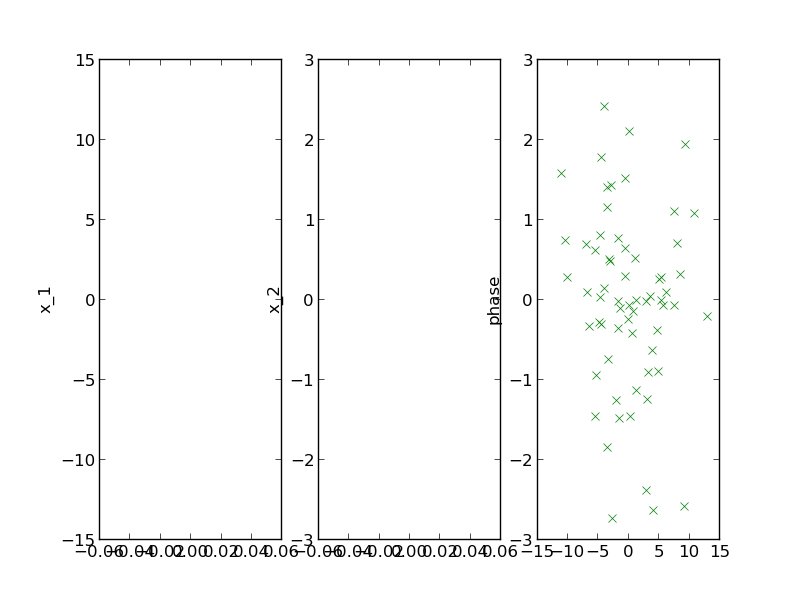
\includegraphics[height=0.3\textheight]{{../../challenge_problem/prelim_analysis/animate/anim_f1_t0.010010}.png}
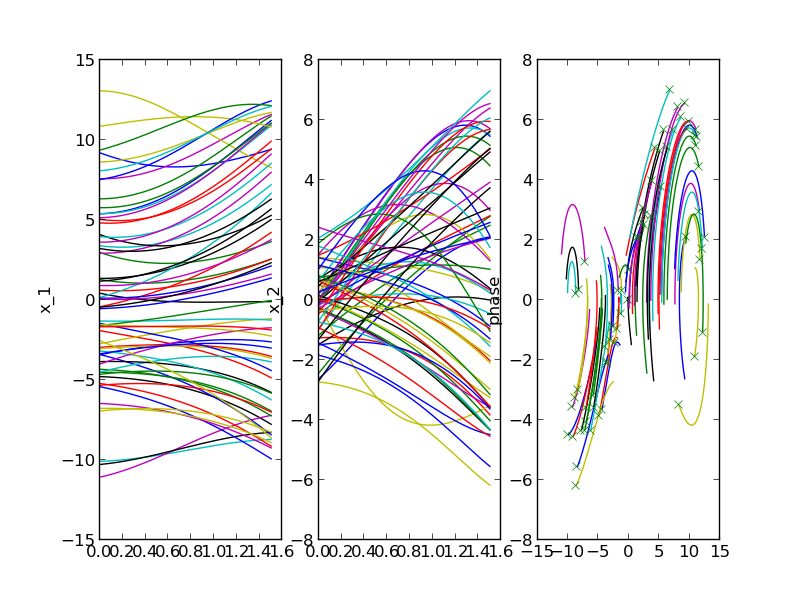
\includegraphics[height=0.3\textheight]{{../../challenge_problem/prelim_analysis/animate/anim_f151_t1.511512}.png}
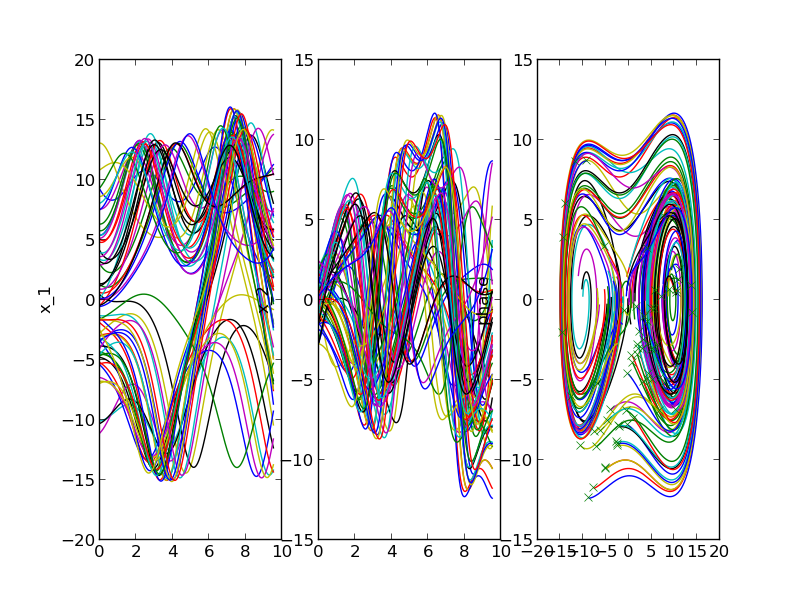
\includegraphics[height=0.3\textheight]{{../../challenge_problem/prelim_analysis/animate/anim_f951_t9.519520}.png}
\caption{Figures showing the development of the distribution. Left: time hsitory of position. Center: time history of speed. Right: phase portrait of system, with 'x' used to indicate the current condition of the state. Top: Initially Gaussian points with position variance $0.1$ and speed variance $1.0$. Middle: Condition of the sustem after 1.5 seconds; clear separation between points in the phase portratit is visible. Bottom: Long-term development of the system after 9.5 seconds, showing the unforced motion of points.}
\label{fig:bifurcation_animate_1}
\end{figure}

%A test for multimodality is performed using smoothed kernel density estimates (KDEs). The procedure is outlined briefly in the following subsection.

\subsection{Test for multimodality}

The test for multimodality is Silverman's\cite{silverman}; for implementation, reference is also made to \cite{adereth}. The KDE is a method of nonparametric estimation of a density function. The KDE for a particular kernel $K(.)$ is defined for samples $\chi = \{ X_1,X_2,...X_n \}$ as follows:

\begin{equation}
\hat{f}(x;h) = \frac{1}{nh} \sum_{i=1}^{n} K(\frac{x-X_i}{h})
\label{eq:kde_def}
\end{equation}

In Eq. \ref{eq:kde_def}, $h$ is a smoothing parameter. The kernel function in general may take different forms, but the Silverman test uses a univariate normal distribution. For a given data set $\chi$, the number of modes in the data (determined by the number of local extrema) is monotonically decreasing with the value of the smoothing parameter, according to Silverman\cite{silverman}. So, a simple binary search can be used to determine the critical smoothing parameter $h_{crit}$ at which the KDE has a particular number of modes. The objective of the test is to if the distribution of the position and velocity states at a fixed time is unimodal; therefore, the smoothing parameter for which the KDE has only one extrema is sought.

One additional procedure is used in the test; smoothed bootstrap sampling. The test works by evaluating the significance of the null hypothesis that the underlying distribution is unimodal. If the significance is too small, the null hypothesis is rejected, and the distribution is assumed to be multimodal. Smoothed bootstrap sampling is used to evaluate the significance level. Bootstrap samples $X_i^*$ are drawn from the original data set $\chi = \{ X_1,X_2,...X_n \}$ as follows:

\begin{equation}
X_i^* = \frac{X_{j(i)} + h\epsilon_i}{\sqrt{1+h^2/\sigma^2}}, i \in [1,\dots,n]
\label{eq:smoothedBootstrap}
\end{equation}

In Eq. \ref{eq:smoothedBootstrap}, the sample $X_{j(i)}$ is selected uniformly with replacement. $\sigma$ is the sample standard deviation of the data. $\epsilon_i$ is a normally distributed random variable with uniform variance. The smoothed bootstrap samples are used to evaluate the null hypothesis that the distribution is unimodal with a critical KDE parameter $h_{crit}$; $N_b$ sets are drawn using smoothed bootstrap sampling, and the number of maxima of the resulting KDE with $h_{crit}$ are tabulated. The fraction of sets with only one maximum is taken to be the significance level of the null hypothesis.

The test procedure is summarized as follows:

\begin{enumerate}
\item Simulate $N_p$ Monte Carlo simulations for a fixed time
\item For each time $t^*$ in the simulation outputs:
\begin{enumerate}
	\item Collect the $N_p$ state values at $t = t^*$
	\item Compute the critical smoothing parameter $h_{crit}$ for which the KDE is unimodal
	\item Evaluate the probability that the distribution has one mode
	\begin{enumerate}
		\item Perform smoothed bootstrap sampling from the critical KDE $N_b$ times
		\item For each of the $N_b$ samples:
		\begin{enumerate}
			\item Evaluate the KDE with the critical smoothing parameter for the current sample. Record the number of modes.
		\end{enumerate}
		\item The fraction of unimodal KDEs is taken as the P-value for the test.	
	\end{enumerate}
\end{enumerate}
\end{enumerate}

\bibliographystyle{plain}
\bibliography{ref}

\end{document}
